% Figure 1, the method overview: data, the shared recipe over three backbones, the two post-pretraining
% operations, and the evaluation. Drawn at the printed width of the text column (5.5 in, \linewidth in
% main.tex), so \includegraphics[width=\linewidth]{figures/fig1_method.pdf} prints every label at 7 or 8 pt.
%
% Build (from paper/figures):  pdflatex fig1_method.tex && pdftoppm -r 300 -png -singlefile fig1_method.pdf fig1_method
%
% Every fact is read from the code; the source of each is noted beside the panel that draws it. Colour carries
% one meaning throughout: blue marks the four training maps and what is fit on them, orange the thirteen
% unseen arenas and what is fit on one of them, grey what stays frozen.
\documentclass[border=0pt]{standalone}
% no creation date or trailer id, so an unchanged figure rebuilds byte-identical (as make_adapt_figures.save does);
% no object streams, so the page box and font names stay readable in the file (paper/fixtures/test_fig1_method.py)
\pdfinfoomitdate=1\pdftrailerid{}\pdfsuppressptexinfo=-1\pdfobjcompresslevel=0
\usepackage{amsmath,amssymb}
\usepackage{tikz}
\usetikzlibrary{arrows.meta,calc,backgrounds,patterns}
% the CoRL style's text fonts (corl_2026.sty: \rmdefault ptm, \sfdefault phv); math stays Computer Modern, as in the paper
\renewcommand{\rmdefault}{ptm}
\renewcommand{\sfdefault}{phv}

% palette: the neutral inks and the first two categorical slots of paper/make_adapt_figures.py
\definecolor{ink}{HTML}{0B0B0B}
\definecolor{sec}{HTML}{52514E}
\definecolor{muted}{HTML}{898781}
\definecolor{shade}{HTML}{E1E0D9}
\definecolor{trainc}{HTML}{2A78D6}   % training maps 2 to 5, and what is fit on them
\definecolor{unseenc}{HTML}{EB6834}  % unseen arenas 1 and 6 to 17, and what is fit on one of them
\definecolor{panel}{HTML}{F5F4F1}

\newcommand{\fs}{\fontsize{7}{8.2}\selectfont}
\newcommand{\fh}{\fontsize{8}{9.6}\selectfont\bfseries}

\begin{document}
\fs\hyphenpenalty=10000\exhyphenpenalty=10000
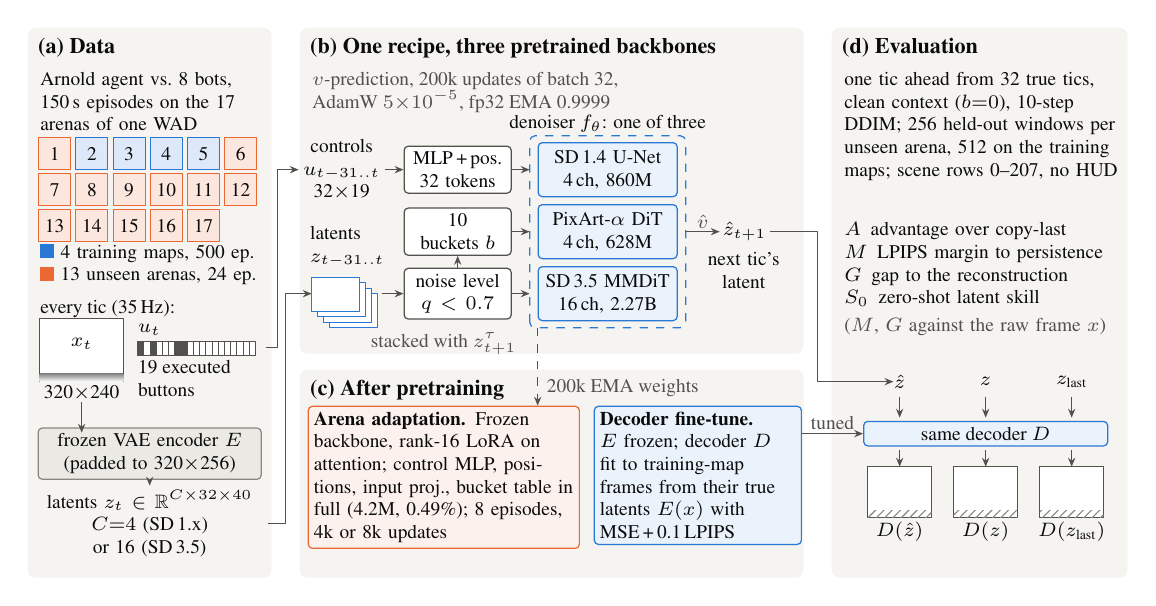
\begin{tikzpicture}[x=1in, y=1in, line join=round,
  every node/.style={font=\fs, text=ink, inner sep=1.5pt},
  flow/.style={-{Stealth[length=3.2pt,width=2.6pt]}, line width=0.55pt, draw=sec},
  lab/.style={font=\fs, text=sec, inner sep=1pt},
  box/.style={draw=sec, line width=0.45pt, rounded corners=1.5pt, fill=white, inner sep=2pt, align=center},
  frozen/.style={box, draw=muted, fill=shade!70},
  trained/.style={box, draw=trainc, fill=trainc!10},
  arena/.style={box, draw=unseenc, fill=unseenc!9},
  head/.style={font=\fh, anchor=north west, inner sep=0pt},
  cell/.style={draw=#1, fill=#1!16, line width=0.4pt, minimum width=0.16in, minimum height=0.16in, inner sep=0pt},
]
\def\H{2.75}
\useasboundingbox (0,0) rectangle (5.5,\H);

% ---------------------------------------------------------------------------------------- panel tiles
\begin{scope}[on background layer]
  \fill[panel, rounded corners=3pt] (0,0) rectangle (1.22,\H);
  \fill[panel, rounded corners=3pt] (1.36,1.12) rectangle (3.88,\H);
  \fill[panel, rounded corners=3pt] (1.36,0) rectangle (3.88,1.04);
  \fill[panel, rounded corners=3pt] (4.02,0) rectangle (5.5,\H);
\end{scope}

% ============================================================================ (a) data
% record_arnold.py:14 and :373 (320x240 RGB with HUD; 150 game-seconds); scripts/spiderman/record_dense.sh:28-31
% and :51 (full_deathmatch WAD; maps 2,3,4,5; --n_bots 8); release/dense_split.json (arenas = maps 2-5, training
% ids 0:2000, i.e. 500 per map); adapt_split.py:66-67 (16 adaptation and 8 held-out episodes per unseen arena);
% transitions.py:32 and docs/cards/arnold/buttons.json (19 executed buttons); encode_parquet.py:155-170 and :252
% (240 rows padded to 256, frozen encoder's posterior mean, C x 32 x 40); backbones.py:60 and :68 (4 or 16 channels)
\node[head] at (0.05,\H-0.05) {(a) Data};
\node[anchor=north west, align=left, text width=1.14in] at (0.04,\H-0.20)
  {Arnold agent vs.\ 8 bots, 150\,s episodes on the 17 arenas of one WAD};
\foreach \m in {1,...,17} {
  \pgfmathtruncatemacro{\col}{mod(\m-1,6)}
  \pgfmathtruncatemacro{\row}{(\m-1)/6}
  \ifnum\m>1 \ifnum\m<6 \def\cc{trainc}\else\def\cc{unseenc}\fi\else\def\cc{unseenc}\fi
  \node[cell=\cc] at ({0.135+\col*0.186},{\H-0.63-\row*0.18}) {\m};
}
\node[anchor=north west, align=left, text width=1.16in] at (0.04,\H-1.06)
  {{\color{trainc}\rule{5pt}{5pt}} 4 training maps, 500 ep.\\
   {\color{unseenc}\rule{5pt}{5pt}} 13 unseen arenas, 24 ep.};
\node[anchor=north west, align=left] at (0.04,\H-1.34) {every tic (35\,Hz):};
% one recorded tic: the frame (HUD band at the bottom, 32 of 240 rows) and the 19-button executed control
\begin{scope}[shift={(0.06,0.98)}]
  \draw[line width=0.4pt, draw=sec, fill=white] (0,0) rectangle (0.42,0.315);
  \fill[shade] (0,0) rectangle (0.42,0.042);
  \node at (0.21,0.19) {$x_t$};
  \node[anchor=north, inner sep=1pt] at (0.21,0) {320$\times$240};
  \foreach \b [count=\i from 0] in {1,0,1,0,0,0,1,1,0,0,0,0,0,0,0,0,0,0,0} {
    \ifnum\b=1 \def\bc{sec}\else\def\bc{white}\fi
    \draw[line width=0.3pt, draw=sec, fill=\bc] ({0.49+\i*0.031},0.13) rectangle ++(0.031,0.07);
  }
  \node[anchor=south west, inner sep=0pt] at (0.49,0.23) {$u_t$};
  \node[anchor=north west, align=left, inner sep=0pt] at (0.49,0.11) {19 executed\\buttons};
\end{scope}
\node[frozen, text width=1.06in] (enc) at (0.61,0.62) {frozen VAE encoder $E$\\(padded to 320$\times$256)};
\draw[flow] (0.27,0.88) -- (0.27,0.725);
\node[anchor=north, align=center, text width=1.14in] (lat) at (0.61,0.46)
  {latents $z_t\in\mathbb{R}^{C\times32\times40}$\\$C{=}4$ (SD\,1.x) or 16 (SD\,3.5)};
\draw[flow] (enc.south) -- (lat.north);

% ============================================================================ (b) backbone under one recipe
% scripts/spiderman/launch_nexttic.sh:220-222 (context 32, action history 32, noise 0.7 in 10 buckets, batch 32,
% lr 5e-5, v objective, EMA 0.9999 applied every 8 updates); train_wm.py:813-815 (noise_augment, training_loss),
% :427-430 and :845 (fp32 EMA on the CPU); diffusion_v.py:63-65 (v target) and :135-151 (context noise, bucket);
% doom_data.py TicWindowDataset (context C*L x 32 x 40; executed buttons of each context tic); backbones.py:153-181
% (control MLP + learned positions), :236-238 (C(L+1) input channels), the U-Net, PixArt and SD 3.5 wrappers;
% 200k = the snap_0200000 every row is evaluated at (launch_nexttic.sh:113: runs are stopped by hand)
\node[head] at (1.41,\H-0.05) {(b) One recipe, three pretrained backbones};
\node[anchor=north west, align=left, text=sec] at (1.40,\H-0.20)
  {$v$-prediction, 200k updates of batch 32,\\AdamW $5{\times}10^{-5}$, fp32 EMA 0.9999};
% denoiser slot: three interchangeable blocks (parameter counts: paper/appendix.tex tab:recipe)
\node[anchor=south, inner sep=1pt] at (2.90,2.21) {denoiser $f_\theta$: one of three};
\draw[draw=trainc, dashed, line width=0.45pt, rounded corners=2pt] (2.51,1.25) rectangle (3.29,2.21);
\node[trained, text width=0.64in, minimum height=0.27in] (unet) at (2.90,2.04) {SD\,1.4 U-Net\\4\,ch, 860M};
\node[trained, text width=0.64in, minimum height=0.27in] (pix)  at (2.90,1.73) {PixArt-$\alpha$ DiT\\4\,ch, 628M};
\node[trained, text width=0.64in, minimum height=0.27in] (sd35) at (2.90,1.42) {SD\,3.5 MMDiT\\16\,ch, 2.27B};
% row 1: the executed controls of the 32 context tics, one token each
\node[align=center] (u) at (1.57,2.04) {controls\\$u_{t-31..t}$\\32$\times$19};
\node[box, text width=0.48in] (mlp) at (2.15,2.04) {MLP\,+\,pos.\\32 tokens};
\draw[flow] (u.east) -- (mlp.west);
\draw[flow] (mlp.east) -- (2.51,2.04);
% row 3: the 32 context latents, noised at one level q per example, stacked on channels with the noisy target
\foreach \k in {3,2,1,0} {
  \draw[line width=0.4pt, draw=trainc, fill=white] ({1.42+\k*0.03},{1.33-\k*0.026}) rectangle ++(0.24,0.17);
}
\node[anchor=south west, inner sep=0pt, align=left] at (1.41,1.55) {latents\\$z_{t-31..t}$};
\node[box, text width=0.48in] (noise) at (2.15,1.42) {noise level\\$q<0.7$};
\draw[flow] (1.77,1.42) -- (noise.west);
\draw[flow] (noise.east) -- (2.51,1.42);
\node[anchor=north, lab, align=center] at (2.08,1.24) {stacked with $z^{\tau}_{t+1}$};
% row 2: the noise level's bucket
\node[box, text width=0.48in] (bucket) at (2.15,1.73) {10 buckets $b$};
\draw[flow] (noise.north) -- (bucket.south);
\draw[flow] (bucket.east) -- (2.51,1.73);
% output
\draw[flow] (3.29,1.73) -- node[lab, above] {$\hat v$} (3.46,1.73);
\node[anchor=west, inner sep=1pt] (zhat) at (3.46,1.73) {$\hat z_{t+1}$};
\node[anchor=north, align=center, text width=0.56in, inner sep=0pt] at (3.58,1.63) {next tic's latent};

% ============================================================================ (c) after pretraining
% lora.py:44-46 (attention targets; parts control, input_proj, noise_emb) and backbones.py:170-174 (the control
% MLP's position table); adapt_wm.py:84, :88, :504-507 (grid to 4k, lr 1e-4, rank 16, alpha 16); adapt_split.py:69
% (k = 8); results/adapt/*_g8k (the 8k grid); results/adapt/unet200k_arenas13_map07_r16_k8_s0/config.json
% (4,212,544 trained of 863,721,668, 0.49 percent; source weights = the 200k snapshot's EMA);
% finetune_decoder.py:60-74 (encoder frozen, decoder trained) and :601-613 (z = E(x) posterior mean, MSE + w LPIPS),
% w = 0.1 per RESEARCH_CONTEXT 2026-09-27 01:10 and 05:20 (the paper's tuned decoder, vae_decoder_sd1x_mse_lpips);
% the committed launcher scripts/spiderman/decoder_mse.sh:94 passes --lpips-weight 0, so that run's line is not in the repo
\node[head] at (1.41,0.99) {(c) After pretraining};
\draw[flow, dashed] (2.55,1.25) -- (2.55,0.86);
\node[anchor=west, lab] at (2.58,0.95) {200k EMA weights};
\node[arena, anchor=north west, align=left, text width=1.30in] (lora) at (1.40,0.86)
  {\textbf{Arena adaptation.} Frozen backbone, rank-16 LoRA on attention; control MLP, positions, input proj., bucket table in full (4.2M, 0.49\%); 8~episodes, 4k or 8k~updates};
\node[trained, anchor=north west, align=left, text width=0.98in] (dec) at (2.83,0.86)
  {\textbf{Decoder fine-tune.} $E$~frozen; decoder~$D$ fit to training-map frames from their true latents $E(x)$ with MSE\,+\,0.1\,LPIPS};

% ============================================================================ (d) evaluation
% eval_tf.py:643 (one tic), :633 and :479 (clean context, bucket 0), 10 DDIM steps (score_adapt.py:604,
% train_wm.py:1065, rescore_tuned_decoder.sh:93; eval_tf.py:502-505 samples by DDIM), :143-158 (prediction, truth
% and copy-last latent through the same decoder; raw frames for the ceiling), :161-163 (raw persistence), :73 and
% :111-113 (scene rows 0-207);
% adapt_split.py:67-70 (8 held-out episodes x 32 windows = 256 per arena); 512 training-map validation windows
% (eps 6000-6099); paper/FIGURES.md (definitions of A, M, G, S)
\node[head] at (4.07,\H-0.05) {(d) Evaluation};
\node[anchor=north west, align=left, text width=1.40in] at (4.06,\H-0.20)
  {one tic ahead from 32 true tics, clean context ($b{=}0$), 10-step DDIM; 256 held-out windows per unseen arena, 512 on the training maps; scene rows 0--207, no HUD};
\node[anchor=north west, align=left, text width=1.42in] at (4.06,1.80)
  {$A$\,\ advantage over copy-last\\
   $M$\,\ LPIPS margin to persistence\\
   $G$\,\ gap to the reconstruction\\
   $S_0$\,\ zero-shot latent skill\\[2pt]
   {\color{sec}($M$, $G$ against the raw frame $x$)}};
% the three latents through one decoder
\foreach \lbl [count=\i from 0] in {{$\hat z$}, {$z$}, {$z_\text{last}$}} {
  \node[anchor=center, inner sep=0pt] (l\i) at ({4.36+\i*0.43},0.98) {\lbl};
  \draw[flow] ({4.36+\i*0.43},0.905) -- ({4.36+\i*0.43},0.80);
}
\node[trained, minimum width=1.22in] (sd) at (4.79,0.72) {same decoder $D$};
\foreach \lbl [count=\i from 0] in {{$D(\hat z)$}, {$D(z)$}, {$D(z_\text{last})$}} {
  \draw[flow] ({4.36+\i*0.43},0.64) -- ({4.36+\i*0.43},0.555);
  \draw[line width=0.4pt, draw=sec, fill=white] ({4.20+\i*0.43},0.30) rectangle ++(0.32,0.255);
  \fill[pattern=north east lines, pattern color=muted] ({4.20+\i*0.43},0.30) rectangle ++(0.32,0.034);
  \node[anchor=north, inner sep=1pt] at ({4.36+\i*0.43},0.295) {\lbl};
}

% ---------------------------------------------------------------------------------------- cross-panel flows
% latents into the context stack, controls into the control row, the prediction and the tuned decoder into (d)
\draw[flow] (lat.east) -| (1.29,1.42) -- (1.42,1.42);
\draw[flow] (1.19,1.15) -- (1.25,1.15) |- (u.west);
\draw[flow] (zhat.east) -- (3.95,1.73) |- (l0.west);
\draw[flow] (dec.east |- sd.west) -- node[lab, above] {tuned} (sd.west);
\end{tikzpicture}
\end{document}
